\subsection{بررسی عملكرد کنترل‌کننده در حضور نويز اندازه‌گیری}\label{roll_noise}

در این بخش عملکرد کنترل‌کننده در حضور نویز (نویز تصادفی حول نقطه صفر و با انحراف معیار دو صدم) وارد بر تمامی مقادیر  اندازه‌گیری‌شده‌ی سنسور، مورد بررسی قرار می‌گیرد. فرکانس تولید نویز در شبیه‌سازی ۵۰ هرتز در نظر گرفته شده‌است.
% در این بخش به بررسی عملکرد چهارپره در حضور کنترل‌کننده \lr{LQR} پرداخته می‌شود. در شبیه‌سازی برای بهینه‌سازی ضرایب وزنی \lr{LQR} از روش بهینه‌سازی
%\lr{TCACS} \cite{Karimi2010}
%استفاده شده‌است.
\begin{figure}[H]
	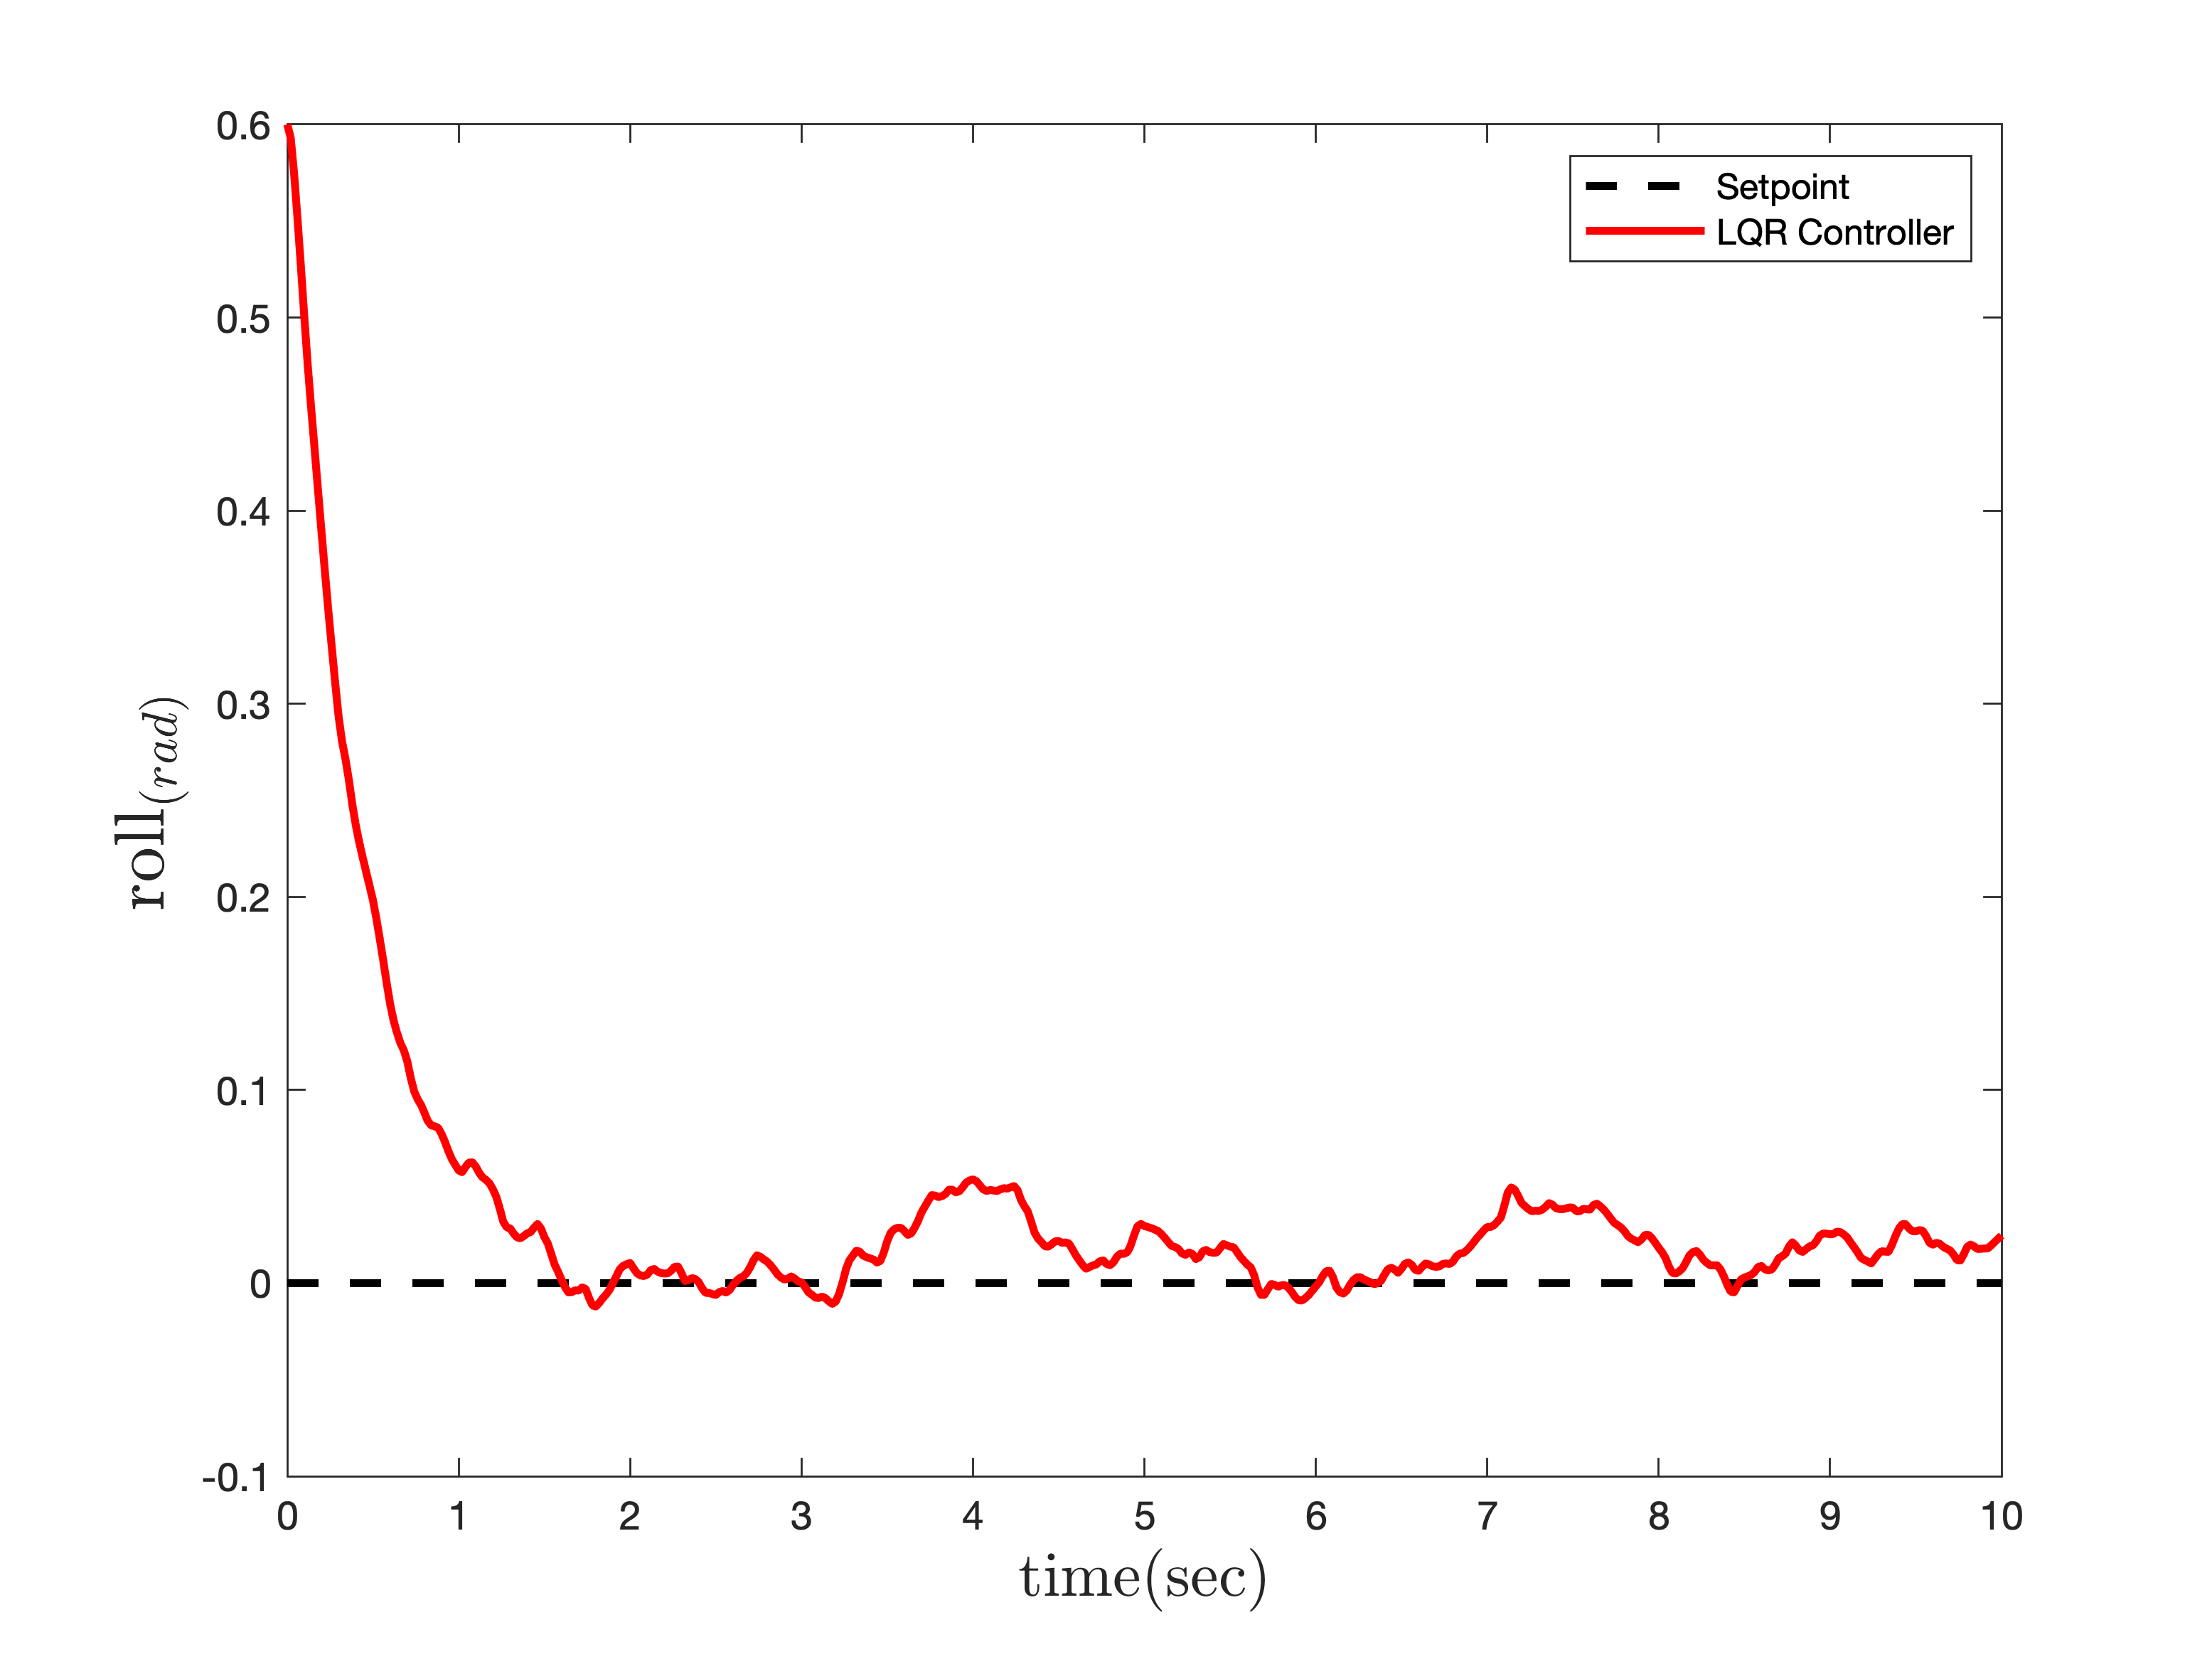
\includegraphics[width=.48\linewidth]{../Figures/MIL/LQR/Roll/lqr_roll.png}
	\centering
	\caption{عملكرد کنترل‌کننده  \lr{LQR} در کنترل زاويه رول با حضور نويز اندازه‌گیری}
	\label{lqr_roll_figure_simulation_n}
\end{figure}
\begin{figure}[H]
	\centering
	\subfigure[موتور شماره دو]{
		\centering
		\includegraphics[width=.45\linewidth]{../Figures/MIL/LQR/Roll/lqr_roll_Omega_2.png}
	}
	\subfigure[موتور شماره چهار]{
		\centering
		\includegraphics[width=.45\linewidth]{../Figures/MIL/LQR/Roll/lqr_roll_Omega_4.png}
	}
	\caption{‫‪فرمان کنترلی موتورهای دو و چهار در کنترل زاویه رول با حضور نويز اندازه‌گیری}
\end{figure}


\بدون‌تورفتگی همانطور که از شکل
\ref{lqr_roll_figure_simulation_n}
مشخص است، عملکرد کنترل‌کننده \lr{LQR} در برابر نویز اندازه‌گیری ضعیف است و خروجی دارای نوسان است.



\begin{figure}[H]
	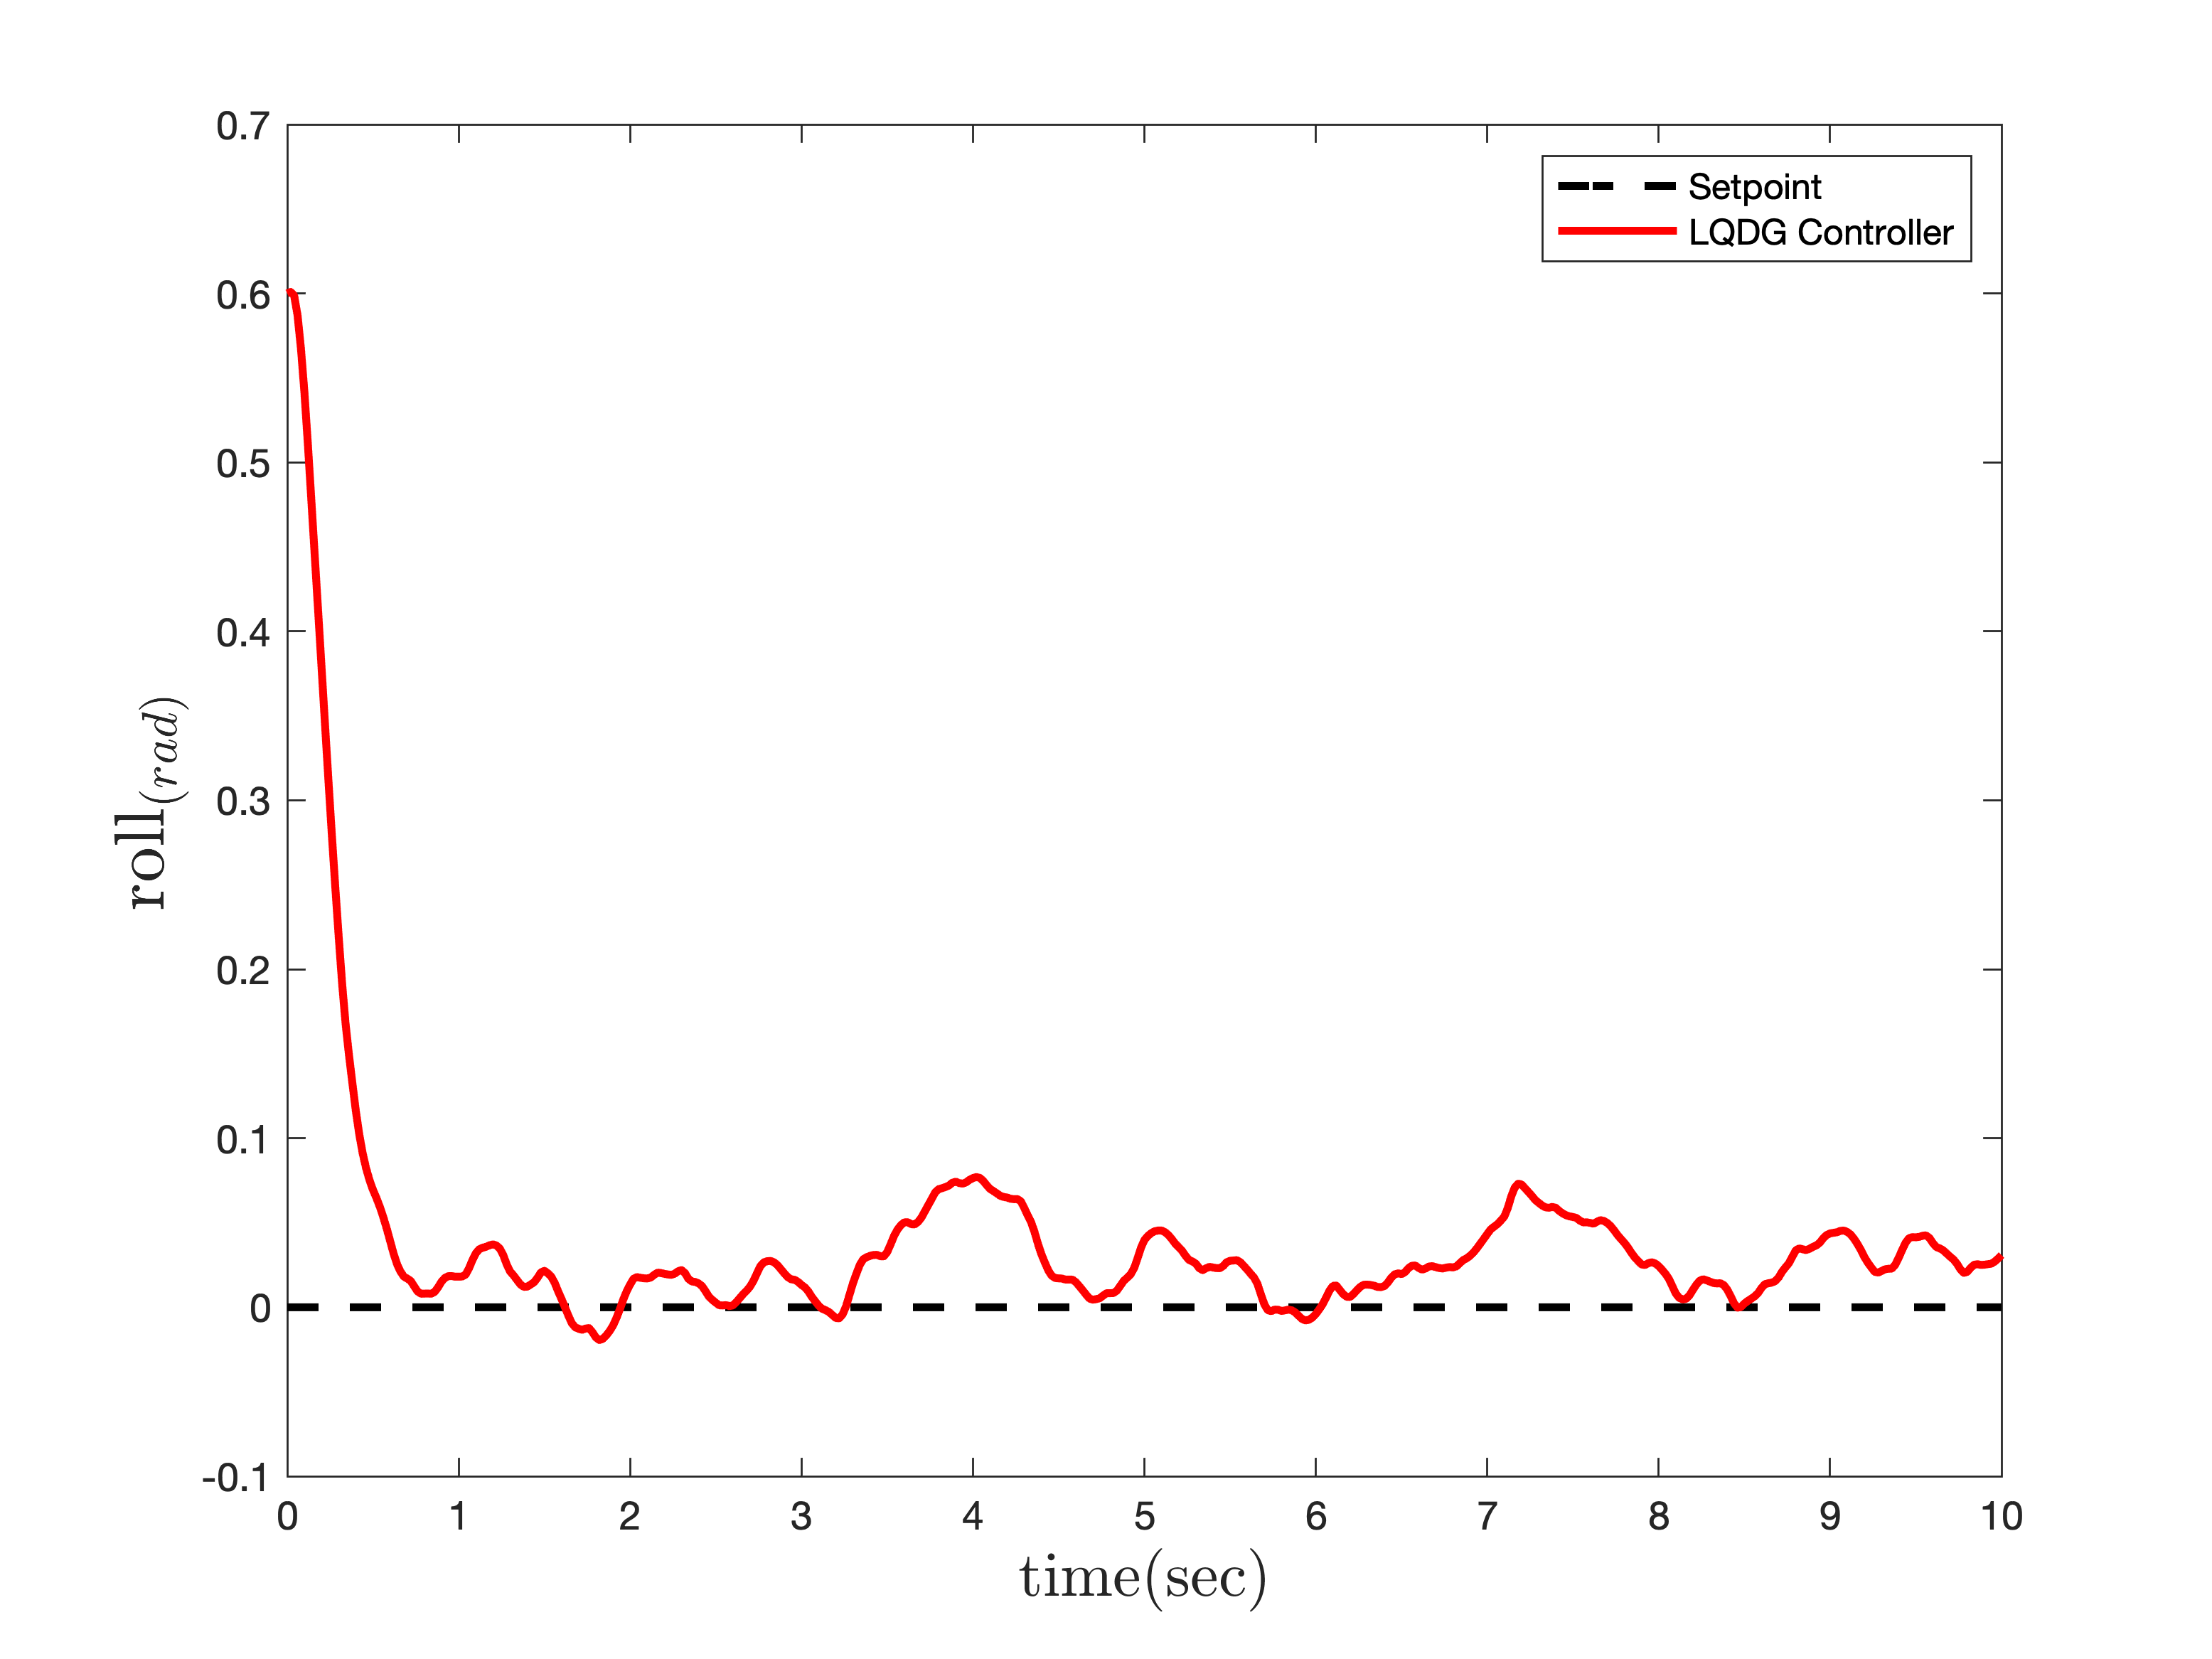
\includegraphics[width=.48\linewidth]{../Figures/MIL/LQDG/Roll/lqdg_roll.png}
	\centering
	\caption{عملكرد کنترل‌کننده  \lr{LQDG} در کنترل زاويه رول با حضور نويز اندازه‌گیری}
	\label{lqdg_roll_fig_simulation_n}
\end{figure}
\begin{figure}[H]
	\centering
	\subfigure[موتور شماره دو]{
		\centering
		\includegraphics[width=.45\linewidth]{../Figures/MIL/LQDG/Roll/lqdg_roll_Omega_2.png}
	}
	\subfigure[موتور شماره چهار]{
		\centering
		\includegraphics[width=.45\linewidth]{../Figures/MIL/LQDG/Roll/lqdg_roll_Omega_4.png}
	}
	\caption{‫‪فرمان کنترلی موتورها در کنترل زاویه رولبا حضور نويز اندازه‌گیری}
\end{figure}
\بدون‌تورفتگی همانطور که از شکل
\ref{lqdg_roll_fig_simulation_n}
مشخص است، عملکرد کنترل‌کننده \lr{LQDG} در برابر نویز اندازه‌گیری ضعیف است و خروجی دارای نوسان است.





\begin{figure}[H]
	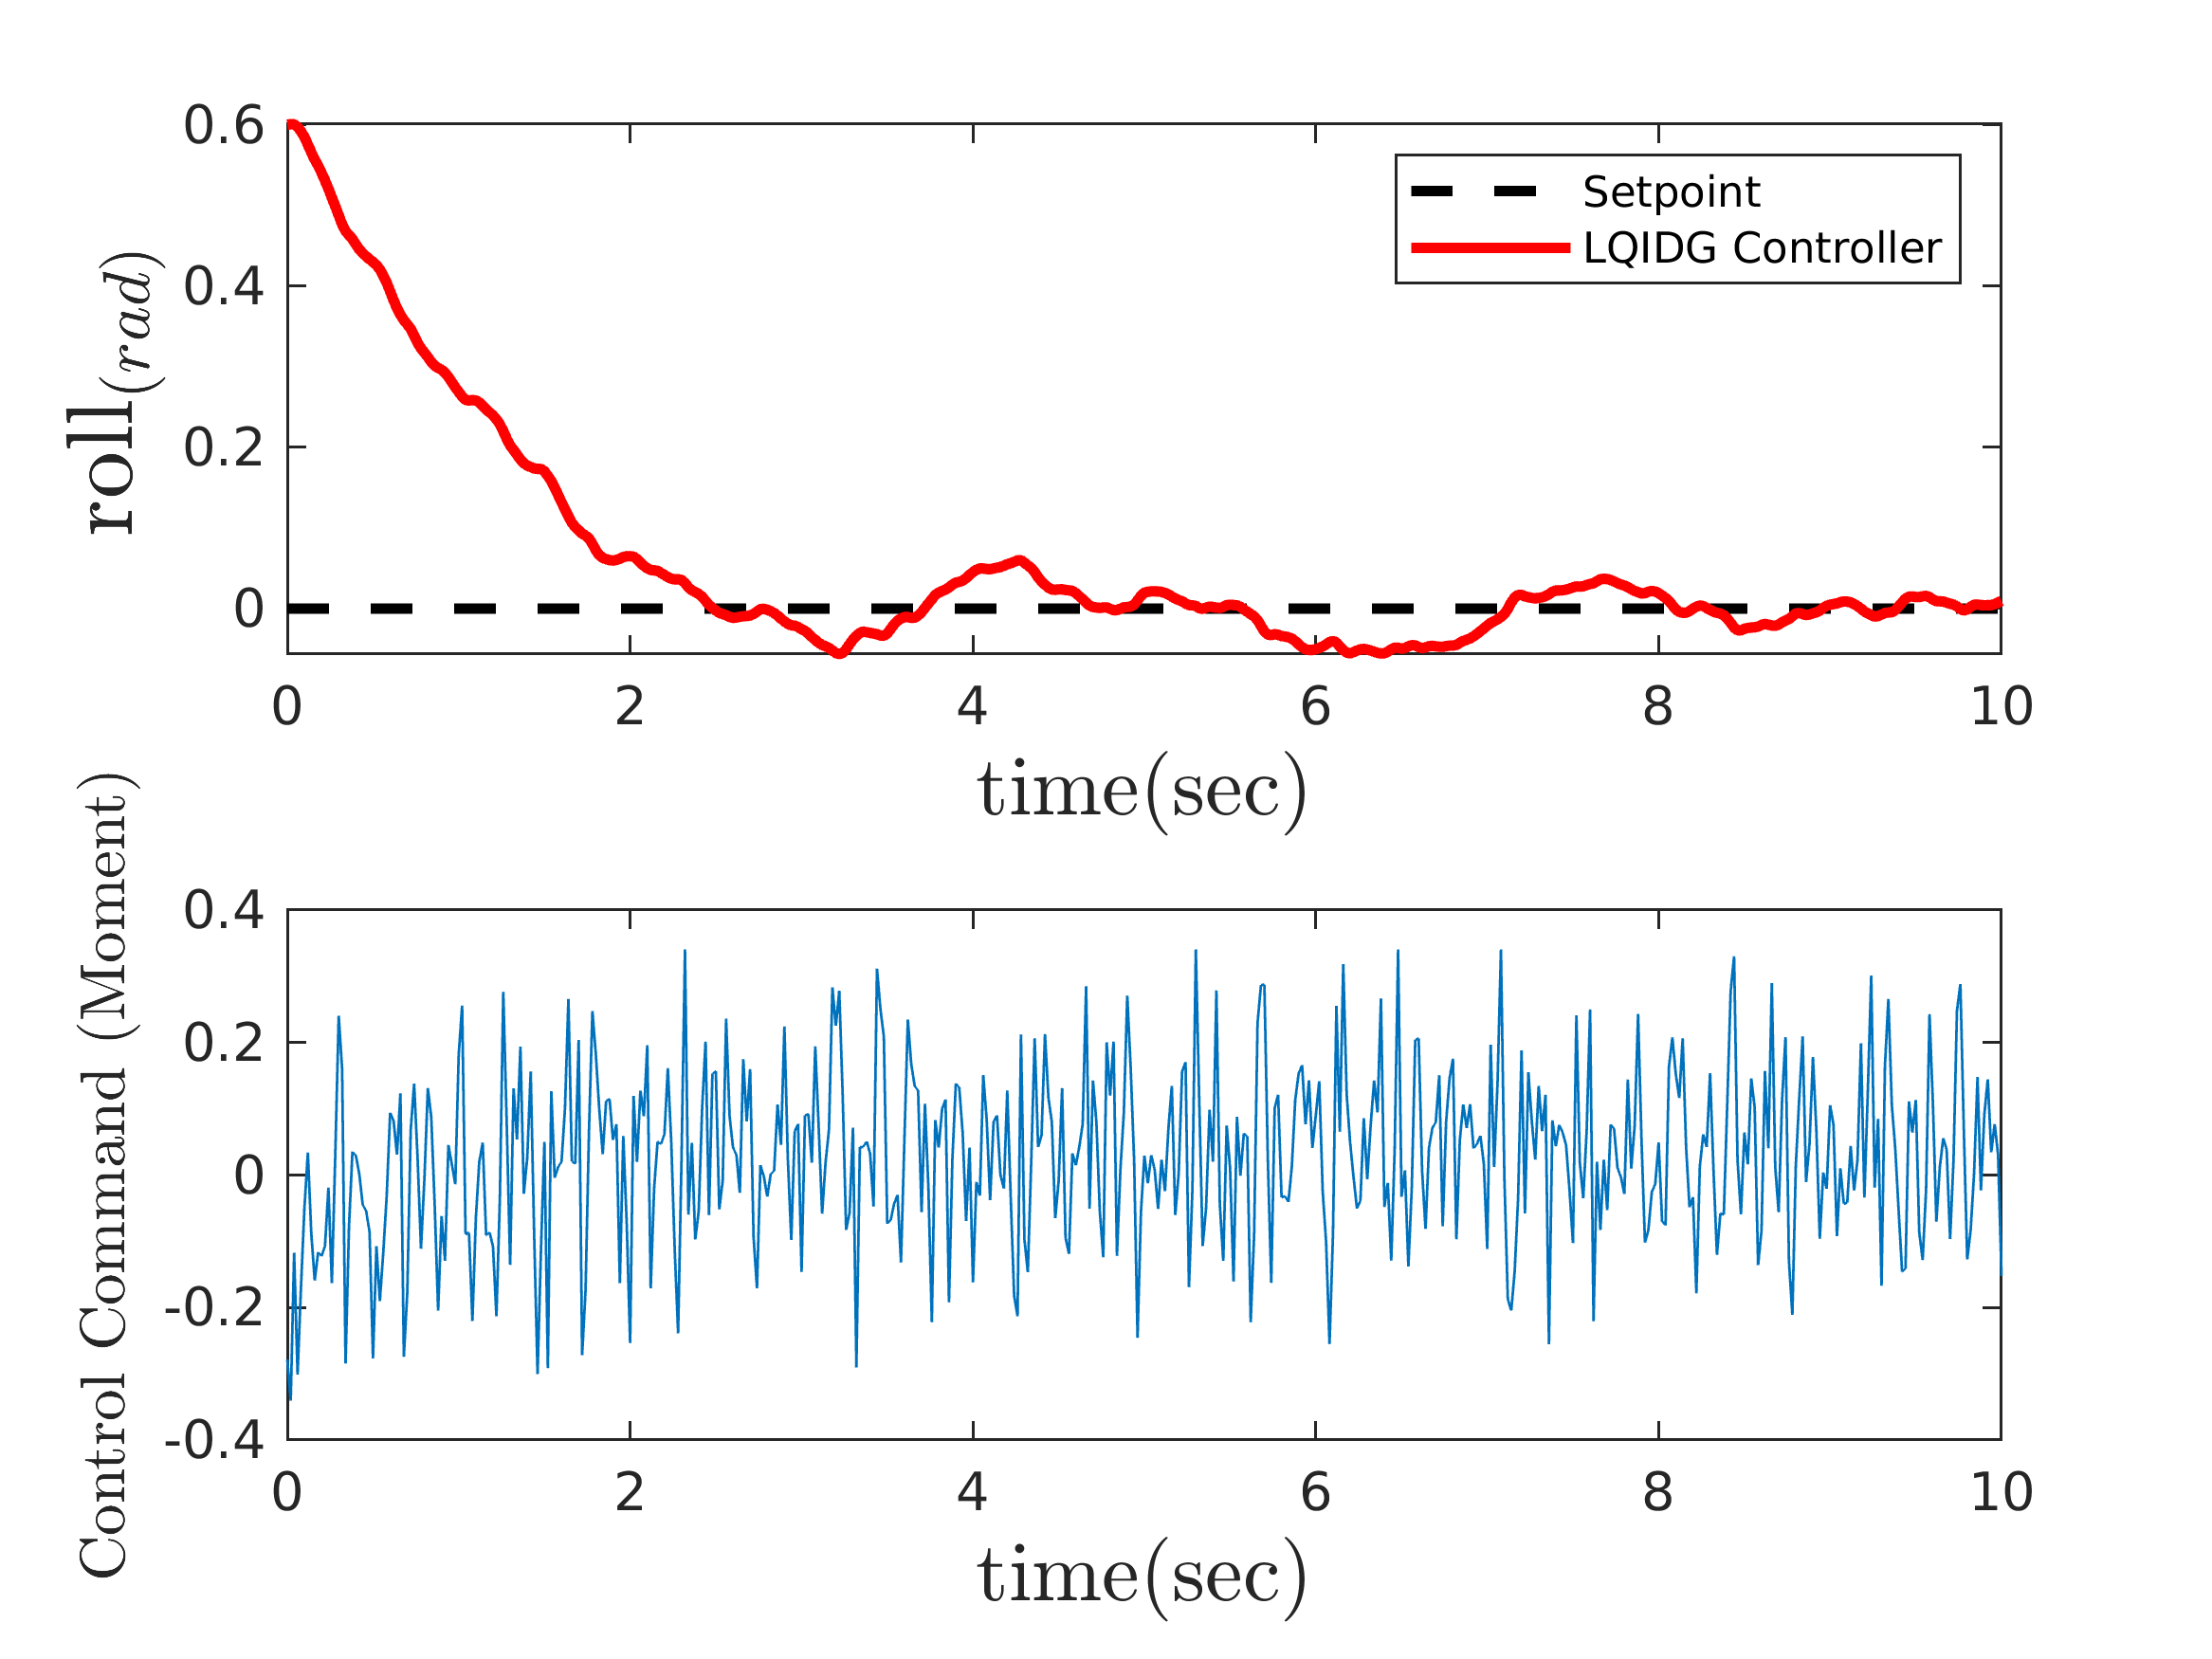
\includegraphics[width=.48\linewidth]{../Figures/MIL/LQIDG/Roll/lqidg_roll.png}
	\centering
	\caption{عملكرد کنترل‌کننده  \lr{LQIDG} در کنترل زاويه رول با حضور نويز اندازه‌گیری}
	\label{lqidg_roll_fig_simulation_n}
\end{figure}
\begin{figure}[H]
	\centering
	\subfigure[موتور شماره دو]{
		\centering
		\includegraphics[width=.45\linewidth]{../Figures/MIL/LQIDG/Roll/lqidg_roll_Omega_2.png}
	}
	\subfigure[موتور شماره چهار]{
		\centering
		\includegraphics[width=.45\linewidth]{../Figures/MIL/LQIDG/Roll/lqidg_roll_Omega_4.png}
	}
	\caption{‫‪فرمان کنترلی موتورهای دو و چهار در کنترل زاویه رول با حضور نويز اندازه‌گیری}
\end{figure}
\بدون‌تورفتگی همانطور که از شکل
\ref{lqidg_roll_fig_simulation_n}
مشخص است، عملکرد کنترل‌کننده \lr{LQDG} در برابر نویز اندازه‌گیری خوب است و خروجی نوسان ندارد.